%
% problemstellung.tex -- Beispiel-File für die Beschreibung des Problems
%
% (c) 2020 Prof Dr Andreas Müller, Hochschule Rapperswil
%
\section{Folgerungen
\label{steps:section:folgerungen}}
\rhead{Folgerungen}
Schrittweitensteuerungen existieren in diversen Variationen, doch alle haben das selbe Ziel, nämlich
das gesuchte Resultat mit möglichst wenig Schritten und mit der erforderlichen Genauigkeit zu berechnen.
Nur dank der Schrittlängensteuerung ist es überhaupt möglich, bei Simulationsprogrammen wie Spice (Simulator für elektronische Schaltungen)
innerhalb nützlicher Zeit ein Ergebnis zu haben. Zur Illustration des Vorteils einer Schrittweitensteuerung dient der Graph~\ref{buch:steps:beispielfuerssc}.
Dabei wird eine Annäherung an $y(1-\varepsilon)$ der Differenzialgleichung $y'=e^y$ mit $y(0)=0$ berechnet.

\begin{figure}
    \centering
    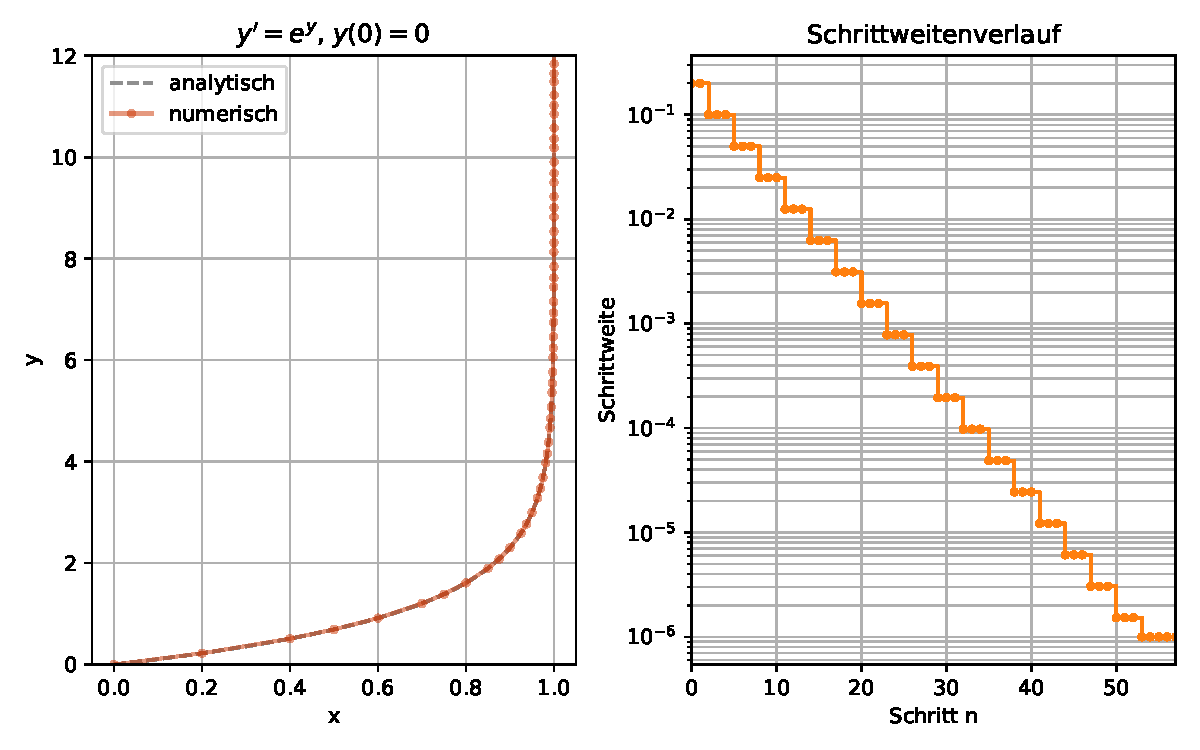
\includegraphics[width=\textwidth]{papers/steps/img/example_for_ssc.pdf}
    \caption{Visualisierung des Vorteils einer Schrittweitensteuerung anhand der Berechnung einer Annäherung für
    $y(1-\varepsilon)$ mit der Gleichung $y'=e^y$ mit $y(0)=0$.
    $\varepsilon$ ist grösser $0$, beispielsweise $10^{-3}$.
    Links: numerische Berechung der DGL $y'=e^y$, jeder Schritt mit einem Punkt hervorgehoben.
    Rechts: Schrittweite (in x-Richtung) während der Berechnung von $y'=e^y$.
    Aufgrund der hohen Steilheit in der Nähe von $x=1$ wird dort eine massiv kleinere Schrittweite benötigt
    als in der Umgebung von $x=0$. Durch die hier angewendete Schrittweitensteuerung lässt sich die benötigte
    Anzahl von Schritten und somit der Rechenaufwand merklich reduzieren.
    \label{buch:steps:beispielfuerssc}}
\end{figure}

Doch auch die Verwendung der Schrittweitensteuerung löst nicht alle Probleme.
So kann es beispielsweise vorkommen, dass kleine Änderungen (relativ zur aktuellen Schrittweite) übersehen werden.
Als Beispiel sei hier die Berechnung der Bahn eines Kometen erwähnt, welcher mit grosser Geschwindigkeit am Mars vorbeifliegt,
wobei dann aufgrund des Übersehens des Gravitationsfeldes des Mars eine falsche Bahn berechnet wird.
Gegen dieses Phänomen lässt sich bei den meisten Applikationen eine maximale Schrittweite festlegen,
doch dadurch steigt zwangsläufig auch der Rechenaufwand.

